\documentclass[12pt]{article}
\usepackage[margin=0.75in]{geometry}
\geometry{a4paper}
\usepackage[T1]{fontenc} % Support Icelandic Characters
\usepackage[utf8]{inputenc} % Support Icelandic Characters
\usepackage{graphicx} % Support for including images
\usepackage{hyperref} % Support for hyperlinks
\usepackage{wrapfig}

\usepackage{algorithm}
\usepackage{algorithmicx}
\usepackage{listings}
\usepackage{color}
\usepackage{siunitx}

\usepackage[svgnames]{xcolor}

\usepackage[spanish]{babel}
\usepackage[latin1]{inputenc}
\usepackage[usenames]{color}

\definecolor{mGreen}{rgb}{0,0.6,0}
\definecolor{mGray}{rgb}{0.5,0.5,0.5}
\definecolor{mPurple}{rgb}{0.58,0,0.82}
\definecolor{backgroundColour}{rgb}{0.95,0.95,0.92}

\usepackage{listings}             % Include the listings-package
\lstdefinestyle{CStyle}{
    backgroundcolor=\color{backgroundColour},   
    commentstyle=\color{mGreen},
    keywordstyle=\color{blue},
    numberstyle=\tiny\color{mGray},
    stringstyle=\color{red},
    basicstyle=\footnotesize,
    breakatwhitespace=false,         
    breaklines=true,                 
    captionpos=b,                    
    keepspaces=true,                 
    numbers=left,                    
    numbersep=5pt,                  
    showspaces=false,                
    showstringspaces=false,
    showtabs=false,                  
    tabsize=2,
    language=C
}


%------------------------------------------------------------------
% TITLE
%------------------------------------------------------------------

\title{
\centerline{
    
\includegraphics[width=75mm]{unsa.png}}
    \vspace{0.5 cm}
        Programación de Sistemas - Laboratorio - Grupo B
        \\
        \\
        \\
        \textbf{Práctica Laboratorio N7} 
        \large  
        \\
        %SC-T-718-ATSR,Automatic Speech Recognition, 2019-1 
        %\\ 
        \small Universidad Nacional de San Agustín - Escuela Profesional de Ingeniería de Sistemas, Arequipa, Perú 
  }

\author{
    Carlos Alberto Mestas Escarcena
    \\
    \texttt{cmestas@unsa.edu.pe}
}

\date{Junio 2020}

\begin{document}

\maketitle

El desarrollo de este informe se puede encontrar en el repositorio de \textcolor{blue}{
    \href{https://github.com/CarlosMestas/Programacion_de_Sistemas_Laboratorio_B_Carlos_Mestas_Practica7}{GitHub}}.
    
%%%%1
\section{Ejercicio 1}

\begin{lstlisting}[language=bash,frame=single,style=CStyle]
// Exercise_1.cpp : Desarrollo del ejercicio 1
// Curso: Programacion de Sistemas
// Laboratorio: B
// Autor: Carlos Alberto Mestas Escarcena
// Fecha: 26/06/2020

#include <iostream>
#include <cstring>	

using namespace std;

// Clase para la exepcion
class	MyException	{
public:
	// Almacenara el mensaje de error
	char msg[40];
	MyException(){
		*msg = 0;	
	}
	MyException(const char *msg2) {
		strcpy(this->msg, msg2);
	}
};

// Funcion principal
int	main()	{
	system("color f0");
	double div1; // Dividendo
	double div2; // Divisor
	cout << "Ingrese el dividendo: ";
	cin >> div1;
	try	{
		cout << "Ingrese el divisor: ";
		cin >> div2;
		// En caso de que el divisor sea 0
		if(div2 == 0){
			throw MyException("El divisor no puede ser cero ...");
		}
		// En caso de que se pueda realizar la division
		else {
			cout << "El resultado de la divison es: " << (div1 / div2);
		}
	}
	catch(MyException	e)	{
		cerr <<	"Error:	" << e.msg;
	}
	return	0;
}
\end{lstlisting}

\begin{figure}[h]
    \centering
    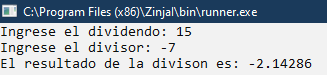
\includegraphics[width=0.5\textwidth]{images/Capture01A.PNG}
    \caption{Ejercicio 1 - Ejecución I}
\end{figure}

\begin{figure}[h]
    \centering
    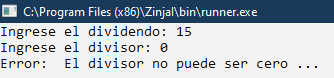
\includegraphics[width=0.5\textwidth]{images/Capture01B.PNG}
    \caption{Ejercicio 1 - Ejecución II}
\end{figure}

\clearpage
\newpage

\section{Ejercicio 2}

\begin{lstlisting}[language=bash,frame=single,style=CStyle]
// Exercise_2.cpp : Desarrollo del ejercicio 2
// Curso: Programacion de Sistemas
// Laboratorio: B
// Autor: Carlos Alberto Mestas Escarcena
// Fecha: 26/06/2020

#include <iostream>
#include <cstring>	

using namespace std;

// Clase para la exepcion
class	MyException	{
public:
	// Almacenara el mensaje de error
	char msg[40];
	MyException(){
		*msg = 0;	
	}
	MyException(const char *msg2){
		strcpy(this->msg, msg2);
	}
};

// Funcion que capturara el error y devolvera al main
void throwExceptionDivisionByZero(double _divisor){
	try{
		if(_divisor == 0){
			throw MyException("El divisor no puede ser cero ...");
		}
	}
	catch(MyException	e)	{
		cerr <<	"Paso del error a la funcion main \n";
		throw;
	}
	
}
// Funcion principal
int	main()	{
	system("color f0");
	double div1; // Dividendo
	double div2; // Divisor
	cout << "Ingrese el dividendo: ";
	cin >> div1;
	try	{
		cout << "Ingrese el divisor: ";
		cin >> div2;
		// En caso de que el divisor sea 0 o negativo
		if(div2 <= 0){
			throwExceptionDivisionByZero(div2);
		}
		// En caso de que se pueda realizar la division
		else {
			cout << "El resultado de la divison es: " << (div1 / div2);
		}
	}
	catch(MyException	e)	{
		cerr <<	"Error en el main:	" << e.msg << "\n";
	}
	return	0;
}
\end{lstlisting}

\begin{figure}[h]
    \centering
    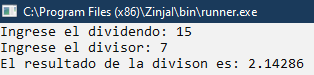
\includegraphics[width=0.5\textwidth]{images/Capture02A.PNG}
    \caption{Ejercicio 2 - Ejecución I}
\end{figure}

\begin{figure}[h]
    \centering
    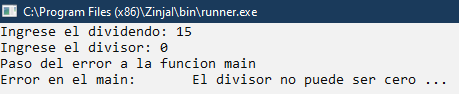
\includegraphics[width=0.5\textwidth]{images/Capture02B.PNG}
    \caption{Ejercicio 2 - Ejecución II}
\end{figure}

\section{Ejercicio 3}

Para los siguientes casos, proponer y explicar dos ejemplos en C++
considerando:

\subsection{Excepciones provocadas por asignación de memoria insuficiente
(generadas por el operador new)}

Por ejemplo si nosotros creamos un arreglo que contenga una cantidad excesiva de elementos, provocaría un error al nosotros empezar asignar valores a los elementos, la memoria sería insuficiente, para ello trabajamos con la excepción $bad\_alloc$.

\subsection{Excepciones por tipos de datos incorrectos (ejemplo, al solicitar un dato
numérico el usuario digita letras)}

Por ejemplo si nosotros tenemos un dato numérico entero, por ejemplo la edad de una persona, pero nosotros al momento de ingresar el dato y se ingresa un texto, entonces automáticamente al valor entero se le asigna el valor de 0, de esta manera nosotros podremos trabajar con la excepción si comprobamos si el valor es igual a 0.

\section{Ejercicio 4}

\begin{lstlisting}[language=bash,frame=single,style=CStyle]
// Exercise_4.cpp : Desarrollo del ejercicio 4
// Curso: Programacion de Sistemas
// Laboratorio: B
// Autor: Carlos Alberto Mestas Escarcena
// Fecha: 26/06/2020

#include <iostream>
#include <cstring>	
#include <math.h>

using namespace std;

// Clase para la exepcion
class	MyException	{
public:
	// Almacenara el mensaje de error
	char msg[40];
	MyException(){
		*msg = 0;	
	}
	MyException(const char *msg2) {
		strcpy(this->msg, msg2);
	}
};

// Funcion principal
int	main() {
	system("color f0");
	double A;
	double B;
	double C;
	cout << "RAINCES CUADRADAS DE UNA ECUACION \n";
	cout << "Ingrese el coeficiente para A: ";
	cin >> A;
	try	{
		// En el caso de que el coeficiente de A sea 0 no se trataria de
		// una ecuacion cuadratica
		if(A == 0){
			throw MyException("El coeficiente A no puede ser 0 ...");
		}
		cout << "Ingrese el coeficiente para B: ";
		cin >> B;
		cout << "Ingrese el coeficiente para C: ";
		cin >> C;
		// Calculamos la determinante
		double D = pow(B,2) - 4 * A * C;
		if(D < 0){
			throw MyException("Sus raices no son reales ...");
		}
		// En caso de que se pueda realizar la division
		else {
			cout << "Raices: \n";
			cout << "X1 = " << (-B + pow(D,0.5)) / 2 << "\n";
			cout << "X2 = " << (-B - pow(D,0.5)) / 2 << "\n";
		}
	}
	catch(MyException	e)	{
		cerr <<	"Error:	" << e.msg;
	}
	return	0;
}
\end{lstlisting}

\end{document}


